\documentclass[a4paper,english, 10pt, twoside]{article}
\usepackage[utf8]{inputenc}
\usepackage[T1]{fontenc}
\usepackage[english]{babel}
\usepackage{epsfig}
\usepackage{graphicx}
\usepackage{amsfonts, amssymb, amsmath}
\usepackage{listings}
\usepackage{float}
\usepackage[top=2cm, bottom=2cm, left=2cm, right=2cm]{geometry}
%\newcommand{\d}{\partial}
%opening
\title{Project 4, FYS4150}
\author{Fredrik E Pettersen\\ fredriep@student.matnat.uio.no}


\begin{document}

\maketitle


\section*{About the problem}

\section*{Notation}
For finite differences I will use the the notation 
\begin{equation*}
 u(t_n,x_i,y_j) = u^n_{i,j}
\end{equation*}
where $t_n = t_0 + n\cdot\Delta t$, $x_i = x_0 +i\cdot\Delta x$ and $y_j = y_0 +j\cdot\Delta y$. Thus it is important not to 
confuse $u^n$ (u to the power of n) with $u^n_{i,j}$ (u evaluated at timestep n and position i,j).
\section*{The algorithm}
We will solve the 1+1 dimensional difusion equation by three different finite differnce schemes in this project. Using the 
standard approximation of the second derivative in space, we use successively more elaborate approximations to the time derivative. 
\subsection*{Forward Euler}
Starting off with the Forward Euler (FE) approximation we get the following scheme
\begin{align*}
 \frac{u^{n+1}_i-u^n_i}{\Delta t} = \frac{u^n_{i+1}-2u^n_i + u^n_{i-1}}{\Delta x^2}
\end{align*}
\begin{equation}\label{FE}
 u^{n+1}_i = \frac{\Delta t}{\Delta x^2}\left(u^n_{i+1}-2u^n_i + u^n_{i-1}\right) +u^n_i
\end{equation}
So to solve the equation all we have to do is loop over the two variables and we are done.\\
\begin{lstlisting}
for n = 0,1, ... , N
    for i = 0,1, ... , N_x
	u_new[i] = dtdx2*(u_prev[i+1]-2*u_prev[i] + u_prev[i-1]) + u_prev[i];
    u_prev = u_new;
end;
\end{lstlisting}
Skriv om trunkeringsfeil her
\subsection*{Backward Euler}
The Backward Euler (BE) approximation gives us a slightly more elaborate scheme seeing at it is an implicit one. The discretization 
gives
\begin{align*}
 \frac{u^{n}_i-u^{n-1}_i}{\Delta t} = \frac{u^n_{i+1}-2u^n_i + u^n_{i-1}}{\Delta x^2} \\
 u^n_i -\frac{\Delta t}{\Delta x^2}\left(u^n_{i+1}-2u^n_i + u^n_{i-1}\right) = u^{n-1}_i \\
 u^n_i\Big(1+2\dfrac{\Delta t}{\Delta x^2}\Big) -u^n_{i-1}\dfrac{\Delta t}{\Delta x^2} - u^n_{n+1}\dfrac{\Delta t}{\Delta x^2} 
 = u^{n-1}_i
\end{align*}
If we insert for a few steps we see that this takes the form of
\begin{align}\label{BE}
 \left(\begin{array}{c c c c c c c c}
        \Big(1+2\dfrac{\Delta t}{\Delta x^2}\Big) & -\dfrac{\Delta t}{\Delta x^2} &0 &\dots & & &0 &0 \\
        -\dfrac{\Delta t}{\Delta x^2} & \Big(1+2\dfrac{\Delta t}{\Delta x^2}\Big) & -\dfrac{\Delta t}{\Delta x^2} &0 &\dots & & &0 \\
        0& \ddots & \ddots & \ddots & 0 & \dots &  &0\\
        0& \dots & & &0&-\dfrac{\Delta t}{\Delta x^2} & \Big(1+2\dfrac{\Delta t}{\Delta x^2}\Big) & -\dfrac{\Delta t}{\Delta x^2}\\
         0& \dots & && &0&-\dfrac{\Delta t}{\Delta x^2} & \Big(1+2\dfrac{\Delta t}{\Delta x^2}\Big) 
       \end{array}\right)\mathbf{u}^n = \mathbf{u}^{n-1} 
\end{align}
\begin{equation*}
 \mathbf{A}\mathbf{u}^n = \mathbf{u^{n-1}}
\end{equation*}

So for each timestep we need to multiply the inverse of $\mathbf{A}$ with a vector $\mathbf{u}^{n-1}$ containig the solution at 
the previous timestep. Looking a bit closer at equation (\ref{BE}) we realize two things. First of all, the matrix 
$\mathbf{A}$ does'nt change at all throughout the computation so we can get away with invertig it once. Second, and perhaps 
more important, we allready have a very efficient solver for this kind of problem from project 1.\\

Skriv noe om trunkeringsfeil her

\subsection*{Crank Nicolson}
Finally, we can use the Crank Nicolson approximation of the time derivative which is a special case of the so called theta -rule 
with $\theta = 0.5$.
\begin{align*}
 \frac{u^n_i - u^{n-1}_i}{\Delta t} = \frac{1}{2\Delta x^2}\Big(u^n_{i+1} -2u^n_{i} + u^n_{i-1}\Big) +\frac{1}{2\Delta x^2}
 \Big(u^{n-1}_{i+1} -2u^{n-1}_{i} + u^{n-1}_{i-1}\Big) \\
 u^n_i -\frac{\Delta t}{2\Delta x^2}\Big(u^n_{i+1} -2u^n_{i} + u^n_{i-1}\Big) = u^{n-1}_i + 
 \frac{\Delta t}{2\Delta x^2}\Big(u^{n-1}_{i+1} -2u^{n-1}_{i} + u^{n-1}_{i-1}\Big)\\
 u^n_i(2+2C) - Cu^n_{i+1} - Cu^n_{i-1} = u^{n-1}_i(2-2C) + Cu^{n-1}_{i+1} + Cu^{n-1}_{i-1}
\end{align*}
where $C = \frac{\Delta t}{\Delta x^2}$. This can also be expressed as a linear algebra problem
\begin{equation}\label{CN}
 (2\mathbf{I}+C\mathbf{B})\mathbf{u}^n = (2\mathbf{I}-C\mathbf{B})\mathbf{u}^{n-1}
\end{equation}
Again we observe that we will need to invert a matrix, but this time we will also need to do a matrix-vector multiplication.
\begin{align*}
 (2\mathbf{I}+C\mathbf{B})\mathbf{u}^n = (2\mathbf{I}-C\mathbf{B})\mathbf{u}^{n-1} = \tilde{\mathbf{u}}^{n-1}\\
 \mathbf{u}^n = (2\mathbf{I}+C\mathbf{B})^{-1}\tilde{\mathbf{u}}^{n-1}
\end{align*}
This is the same problem as we had in the BE case, only with a modified right-hand side
\subsection*{2+1 dimensional diffusion equation}
For simplicity we will only use explicit schemes for the 2+1 dimensional case. That is we will discretize using the FE and 
a centered difference approximation. These are both very straightforward to discretize and implement
\begin{align*}
 \frac{u^{n+1}_{i,j}-u^n_{i,j}}{\Delta t} = \frac{u^n_{i+1,j}-2u^n_{i,j} + u^n_{i-1,j}}{\Delta x^2}+ 
 \frac{u^n_{i,j+1}-2u^n_{i,j} + u^n_{i,j-1}}{\Delta y^2}
\end{align*}
This leads us to the same scheme as in \ref{FE} only with one more dimension.
\begin{equation*}
 u^{n+1}_{i,j} = \frac{\Delta t}{\Delta x^2}\left(u^n_{i+1,j}-2u^n_{i,j} + u^n_{i-1,j}\right) +
 \frac{\Delta t}{\Delta x^2}\left(u^n_{i,j+1}-2u^n_{i,j} + u^n_{i,j-1}\right)+u^n_{i,j}
\end{equation*}


\begin{align*}
 \frac{u^{n+1}_{i,j}-u^{n-1}_{i,j}}{2\Delta t} = \frac{u^n_{i+1,j}-2u^n_{i,j} + u^n_{i-1,j}}{\Delta x^2}+ 
 \frac{u^n_{i,j+1}-2u^n_{i,j} + u^n_{i,j-1}}{\Delta y^2}
\end{align*}


\section*{Analytic solution}
As a comparison we can find the analytic solution to this problem as follows. 
 \begin{align}\label{eq}
  &\frac{\partial u}{\partial t} = D\frac{\partial^2 u}{\partial x^2}, \,\,\,\,\, u(x,0) = u(d,t) = 0\\
  &x\in[0,d],\,\,\,\,\,\, D = d = u(0,t) = 1
 \end{align}
We see right away that the boundary $x=0$ could give us some problems, so we start off with a small trick
$$
u(x,t) = v(x,t) = u(x,t) - u_s(x)
$$
where the $u_s = 1-x$ term is the steady-state solution to equation \ref{eq}. This trick leaves us with new boundary conditions 
un $u(x,t)$ 
$$
v(0,t) = u(0,t) - u_s(0,t) = 1, \;\; u_s(0,t) = 1 \implies u(0,t) = 0
$$
which makes the whole procedure much simpler. We now assume that $u(x,t)$ can be separated into factors 
\begin{align*}
&u(x,t) = F(x)G(t) \implies \frac{\partial u}{\partial t} = \frac{\partial^2 u}{\partial x^2} \to F(x)\frac{\partial G}{\partial t}
= G(t)\frac{\partial^2 F}{\partial x^2}\\
&\frac{1}{G(t)}\frac{\partial G}{\partial t} =-k^2 =  \frac{1}{F(x)}\frac{\partial^2 F}{\partial x^2}
\end{align*}
We start with the simplest of the equations which is the time dependence
\begin{align*}
 \frac{1}{G(t)}\frac{\partial G}{\partial t} =-k^2\\
 G(t) =C e^{-k^2t}
\end{align*}
and leave it like this for now. The x-dependent equation is somewhat more complicated
\begin{align*}
 \frac{1}{F(x)}\frac{\partial^2 F}{\partial x^2} = -k^2 \\
 F(x) = A\sin(kx) + B\cos(kx)
\end{align*}
\begin{align*}
 F(0) = A\sin(0) + B\cos(0) = 0 \implies B= 0\\
 F(d) = A\sin(kd) = 0 \implies k = \frac{m\pi}{d} = \pi m, \;\; A = A_m
\end{align*}
we now combine all the equations to determine $v(x,t)$
\begin{align*}
 v(x,t) = 1-x + \sum\limits_{m=1}^{\infty}B_me^{-(m\pi)^2t}\sin(m\pi x) \\
 v(x,0) = 1-x +\sum\limits_{m=1}^{\infty}B_m\sin(m\pi x)\\
 \implies \int\limits_0^1\sin(m\pi x)\sin(n\pi x)dx = \delta_{mn} = \int\limits_0^1(x-1)\sin(m\pi x)dx = -\frac{2}{m\pi} = B_m
\end{align*}
This gives us the full analytical solution 
\begin{equation}\label{solution}
 v(x,t) = 1-x-\frac{2}{\pi}\sum\limits_{m = 1}^{\infty}\frac{1}{m}e^{-(m\pi)^2t}\sin(m\pi x) 
\end{equation}
which satisfies all initial and boundary conditions.
\section*{Results}


\section*{Stability and precision}

% \begin{figure}[H]
%  \centering
%  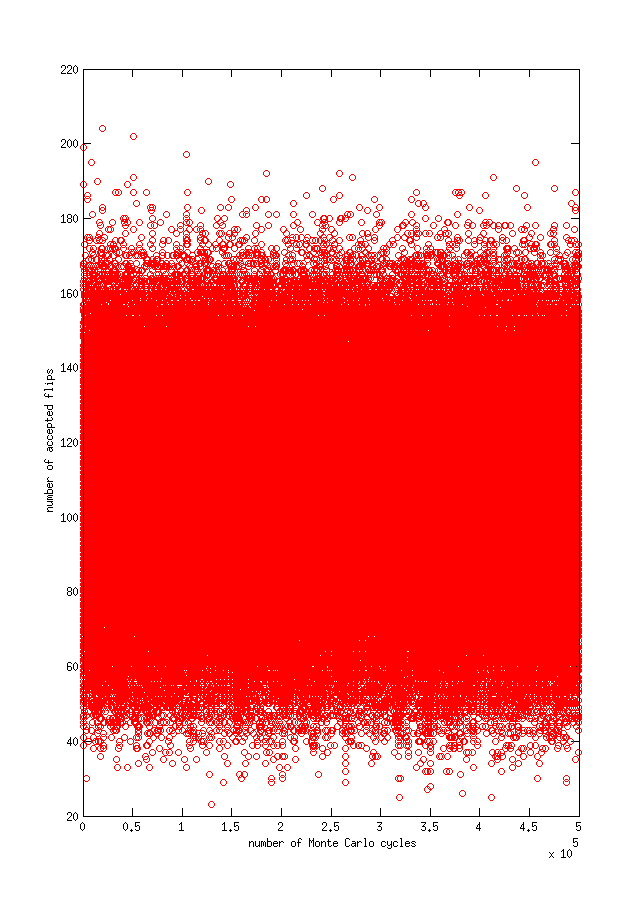
\includegraphics[scale = 0.45]{accepted_flips_temp2dot4.png}
%  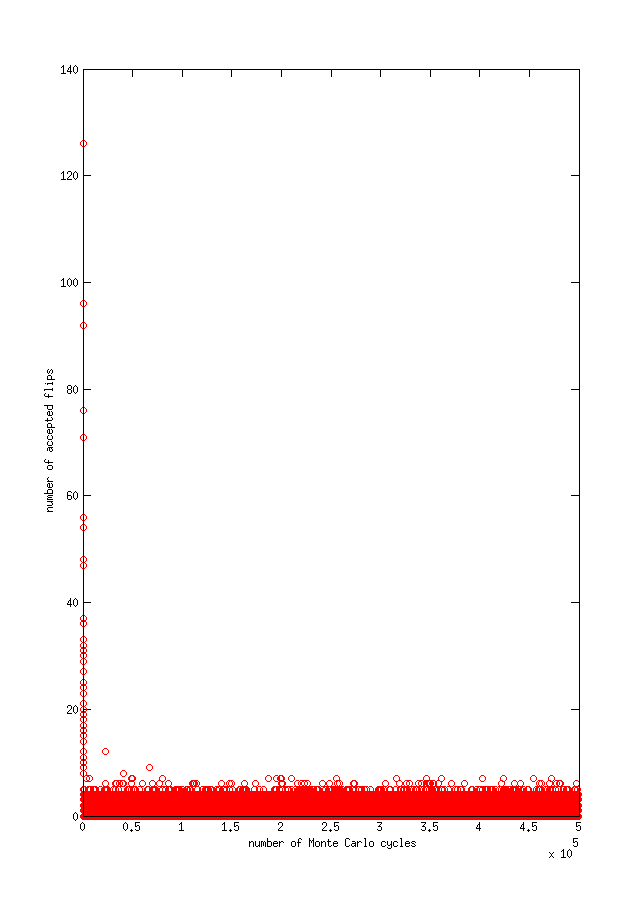
\includegraphics[scale = 0.45]{accepted_flips_temp1.png}
%  \caption{Number of accepted spin flips. T = 2.4 to the left, and T = 1 on the right.}
%  \label{both_accepted_flpis}
% \end{figure}
\section*{Final comments}

\end{document}
